\section{包含已知偶数比特族的母族}
\label{embed:section}

统一构造和已知偶数比特族给出了经过同一基准测量的两个相位方向。本节考察这两个方向能否在保持正四面体几何的同时独立变化。为在完整测量层面比较它们，先用第~\ref{core:framework}~节的记号表达该余弦族。对偶数 $n$，沿用
$E=\{2,4,\ldots,n-2\}$，定义
\begin{equation}
 q_A(z)=\prod_{j\in E}(1-z_j),\qquad d_A(z)=q_A(z)-\delta_{z,0}.
 \label{embed:and-support}
\end{equation}
对角相位 $i^{f_0(z)}e^{i\alpha d_A(z)}$ 恰为 Pauwels 与 Gisin 的偶数比特族~\cite{PauwelsGisin2026}，其参数对应为 $\alpha=\pi\tau/2$。背景仅依赖偶数内部坐标，而表~\ref{core:pullback-table} 中每个字符 $h$ 均含有 $E$ 之外的坐标；翻转该坐标便使背景期望成对消去。此外，I 类有 $q_A(a)=1$，II 类有 $q_A(a)=0$。因此，式~\eqref{core:signal} 给出共同带符号分量 $c_n\cos\alpha$，在 $|\alpha|\le\pi/2$ 上得到 $r=r_E(n)\cos\alpha$。这一论证包括 $n=2$ 时的空乘积 $q_A=1$，以及 $n=4$ 时的 $q_A=1-z_2$。

对偶数 $n\ge8$，该余弦族与统一增强族是同一二维族的坐标截面。令 $d_B=d_n$ 为式~\eqref{core:support} 中的支持，定义
\begin{align}
 D_{\alpha,\beta}(z)&=i^{f_0(z)}e^{i\alpha d_A(z)+i\beta d_B(z)},\notag\\
 M_n(\alpha,\beta)&=C_nD_{\alpha,\beta}H^{\otimes n}.
 \label{embed:measurement}
\end{align}
图~\ref{fig:embedding} 展示这一构造。
\begin{figure*}[tbp]
  \centering
  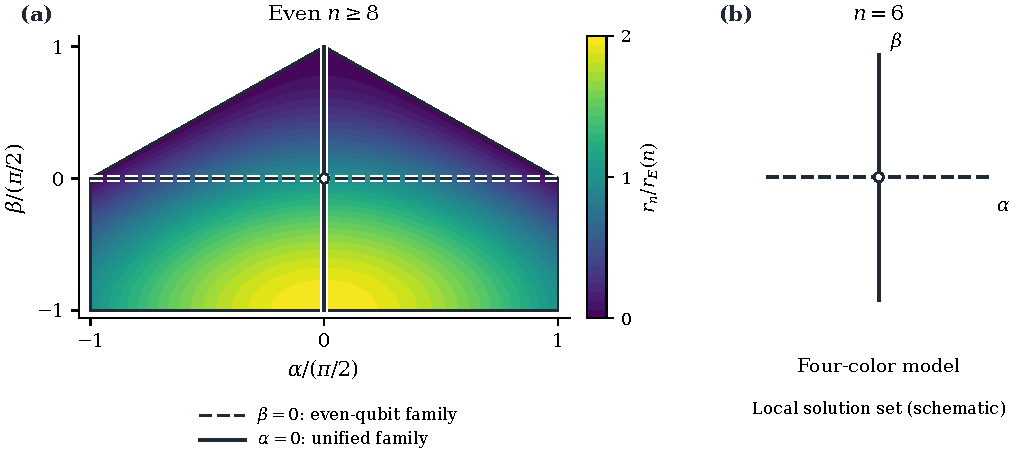
\includegraphics[width=\textwidth]{figures/fig2_embedding.pdf}
  \caption{偶数比特母族的两个精确截面。
  (a) 偶数 $n\geq8$ 的参数域 $\Omega$，颜色表示 $r_n/r_E(n)=\cos\alpha-\sin\beta$。
  虚线截面 $\beta=0$ 逐列恢复已知偶数族，实线截面 $\alpha=0$ 逐列恢复统一增强族。空心圆为共同基点。
  (b) $n=6$ 时四联合颜色加独立零点相位模型的局部解集示意：两支在基点交叉。 绘图代码由 OpenAI Codex（GPT-6）辅助编写，并按文中公式核对。}
  \label{fig:embedding}
\end{figure*}

\begin{theorem}[二维包含]
\label{embed:theorem}
对每个偶数 $n\ge8$，式~\eqref{embed:measurement} 在全部实参数 $\alpha,\beta$ 上定义正交完备测量，其全部种子带符号分量均为
\begin{equation}
 m_n(\alpha,\beta)=c_n(\cos\alpha-\sin\beta).
 \label{embed:component}
\end{equation}
在参数域
\begin{equation}
 \Omega=\left\{(\alpha,\beta): |\alpha|\le\frac\pi2,\quad
 -\frac\pi2\le\beta\le\frac\pi2-|\alpha|\right\}
 \label{embed:domain}
\end{equation}
上，该测量保持式~\eqref{core:bloch-orbit} 的固定局部正四面体，且
\begin{align}
 r_n(\alpha,\beta)&=r_E(n)(\cos\alpha-\sin\beta),\notag\\
 r_n(\Omega)&=[0,2r_E(n)].
 \label{embed:radius}
\end{align}
$\beta=0$ 截面逐列恢复已知偶数比特族，$\alpha=0$ 截面逐列恢复定理~\ref{core:unified-theorem} 的统一增强族。两个参数方向在有序测量投影层面独立。
\end{theorem}

证明的关键在于联合背景消去。令 $u=e^{i\alpha}$、$v=e^{i\beta}$，则施加 $-iC_n$ 之前的种子为
\begin{equation}
 2^{-n/2}\left[\sum_z i^{|z|}u^{q_A(z)}v^{q_B(z)}\ket z
 +(i-uv)\ket{0^n}\right],
 \label{embed:seed}
\end{equation}
其中 $q_B=q_n$。每个 I 类翻转满足 $(q_A(a),q_B(a))=(1,0)$，每个 II 类翻转满足 $(q_A(a),q_B(a))=(0,1)$。因此两类的缺陷贡献相同，因为
\begin{align}
 \operatorname{Re}[-iu^{-1}(i-uv)]
 &=\cos\alpha-\sin\beta,\notag\\
 \operatorname{Re}[-v^{-1}(i-uv)]
 &=\cos\alpha-\sin\beta.
 \label{embed:defect}
\end{align}
I 类翻转不改变 $q_A$，其背景退化为已证明消失的 $q_B$ 背景。对 II 类，将背景和按 AND 差分 $q_A(z)-q_A(z\oplus a)=1,0,-1$ 分为三个扇区。第一扇区的全部偶数内部位为零。当 $n\ge8$ 时，奇数内部块至少含两位；该块上的非常值字符可通过保持奇偶性的双位翻转消去。最后仅剩六个固定四位和，其系数均精确为零。附录~\ref{embed:appendix} 给出完整分类和六个有限恒等式。由此对任意 $n$ 证明式~\eqref{embed:component}，再由轨道公式得到全部约化态。

在 $\Omega$ 上，$\sin\beta\le\cos\alpha$，且 $\cos\alpha-\sin\beta\le2$；$\alpha=0$ 截面已取尽零至二的全部值。两轴的完整测量恒等式直接来自式~\eqref{embed:measurement} 的对角元。为确认参数在取投影后仍然独立，考虑对角输入相位的无穷小变化 $A$：它仅产生列相位，当且仅当存在对角 $B$ 使 $AH^{\otimes n}=H^{\otimes n}B$。Hadamard 矩阵的所有元素均非零，故 $A,B$ 必为同一标量。$(d_A,d_B)$ 在 $0,e_1,e_1\oplus e_2$ 依次取 $(0,0),(1,0),(0,1)$，因此两个方向的非零线性组合不可能为标量。

\begin{proposition}[$n=6$ 时的分支交叉]
\label{embed:six-proposition}
当 $n=6$ 时，式~\eqref{embed:measurement} 的直接叠加具有相同带符号分量，当且仅当 $\sin\alpha\sin\beta=0$。更一般地，允许对 $(q_A,q_B)$ 的四种取值分别赋相位，并独立改变物理零串的相位；在指定 EJM 附近，该模型中的规则测量恰为两条原有单参数分支。
\end{proposition}
此时奇数内部块只有一位。$X_3$ 与 $X_4$ 的归一化背景期望额外出现 $-\sin\alpha\sin\beta/8$，其余分量仍取共同缺陷值。附录~\ref{embed:appendix} 求解了完整的局部颜色方程。因此，$n=6$ 时已有增强族，但这里的二维扩张在局部只保留两条坐标轴的交叉。
